\textbf{Paper Prototype 1.0}

My initial paper prototype, shown in Figure \ref{fig:Paper_Prototype_1.0}, built on the established game structure of manipulating input and output by executing instructions in a player's solution. The objective for each level is displayed at the top left of the screen, the solution space is on the right side, and the remaining area is utilized for visualizing the command execution. This prototype includes a robotic claw that can move horizontally across the top of the main game UI area, and can extend vertically to pick up or drop input values.

\begin{figure}[!hb]
  \caption{Paper Prototype 1.0}
  \label{fig:Paper_Prototype_1.0}
  \centering
  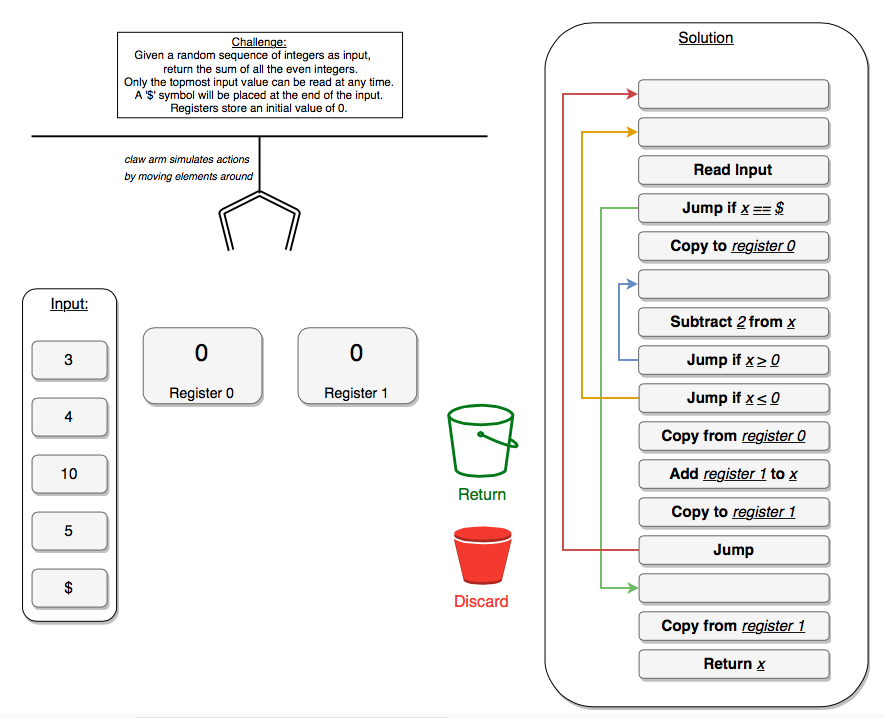
\includegraphics[scale=0.45]{SS_PP1.png}
\end{figure}


\paragraph{Solution Space:} ~\\
The solution space on the right side of the screen is where the player constructs their code-like solution to satisfy the puzzle objectives.
The player must use this space to place a series of instructions that will execute in order.

\paragraph{Instructions/commands:} ~\\
The instructions that are available in this prototype are:
\begin{itemize}
	\item Read Input
	\begin{itemize}
		\item The claw picks up the topmost item from the input.
	\end{itemize}
	\item Jump [If \_\_\_]
	\begin{itemize}
		\item This instruction will point to another line in the solution to jump to while executing.
		\item Optionally, the player may include an If \textit{condition}, so that the jump will only occur if a condition is met.
	\end{itemize}
	\item Copy \_\_\_ \_\_\_
	\begin{itemize}
		\item Copies the current value in the claw to a specified register, or copies the value from a register to the claw.
		\item The first blank can be set to either ``to'' or ``from''
		\item The second value can be set to a specific register
		\item Example: \textit{Copy to register 0}
	\end{itemize}
	\item Add \_\_\_
	\begin{itemize}
		\item Add the value of a specified register to the current value in the claw.
	\end{itemize}
	\item Subtract \_\_\_
	\begin{itemize}
		\item Subtract the value of a specified register from the current value in the claw.
	\end{itemize}
	\item Return
	\begin{itemize}
		\item Place the current value held by the claw into the return bin, and stop executing the instructions.
	\end{itemize}
\end{itemize}


\paragraph{The Claw:} ~\\
As each step of the player's solution is executed, the claw manipulates the data on the board, and the corresponding instructions are highlighted in the solution space.
The claw does all of the work manipulating data as it simulates the player's solution to the puzzle, and it can only hold at most one value at any time.
By having the claw hold a value and manipulate is as specified in the solution, this renders a separate ``current value'' box unnecessary.
The claw can pick up and put down data elements, or it can combine the element it's currently holding with another element to add or subtract values.

\paragraph{Input:} ~\\
Input arrives in a vertical stack that acts like a conveyor belt. The claw will navigate over the input stack, pick up the topmost item, and proceed to manipulate the data.

\paragraph{Registers:} ~\\
Registers are located in the middle of the game board, and they can be used to store data that needs to be set aside while the claw manipulates other data elements.

\paragraph{Discard Bin:} ~\\
Sometimes the current value being held by the claw is no longer needed, so it can be discarded in a trash can towards the bottom right of the screen. This gets rid of the value and can free up space for the claw or registers to hold useful elements.

\paragraph{Puzzle Description:} ~\\
Every puzzle has a clearly defined objective that should result in a single value to return upon completion, similar to a return value of a function in traditional programming. This prototype includes a ``return'' bin next to the discard bin, and the claw will place the final return value in the return bin to end the code execution. If the return value matches the expected value, then the solution was successful, otherwise the solution is incorrect.\\



\textbf{Paper Prototype 2.0: Puzzle Scene Design Concept}

After multiple iterations of prototype testing, team discussions to determine what works and what should be changed, we shared a solid view of how the puzzles should work, the components of included in the puzzles, the complete instruction set, etc.
This prototype was designed to present a possible view of what the entire level will look like, where the components are placed, how they interact with each other on screen, etc.

\todo{Add diagram of prototype and reference above}



\paragraph{Menu Bar:} ~\\
The menu bar stretches across the top of the screen. This contains the name of the current level, along with some buttons to the right.
The Menu button will pause the game and bring up a pause menu, which will present the player with options to exit the puzzle, change game options, or resume the game.
The Help button can be pressed to give useful hints or tips for solving the puzzle if the player is struggling.


\paragraph{Level Description:} ~\\
Below the top menu bar is a section for the the description of the current level objectives. This will contain text that explains the current puzzle in a concise manner.


\paragraph{Solution Space:} ~\\
Similar to previous prototypes, the solution space on the right side is where the player constructs a solution to solve the puzzle objectives. This space includes a scrollbar on the right side to navigate long solutions.


\paragraph{Instruction Set:} ~\\
Below the solution space is the set of instructions the player can use for the current level.
The player can drag and drop these instructions into the solution space to construct their solution.
Dragging an instruction from the set creates a new instance of that instruction, meaning that the instruction does not get removed from the instruction set.
If the player clicks on an instruction, a description of that instruction will appear on the screen to remind the player what the instruction does and how to use it.


\paragraph{Game Space:} ~\\
The majority of the screen will be the game space, which contains the remaining elements which are explained below. The game space is where the remaining components interact to visually simulate the steps as the player's solution is executed.


\paragraph{The Claw:} ~\\
As each step of the player's solution is executed, the claw moves data between game components.
The claw moves horizontally along the top of the game space, and can expand/retract to reach components below it.
The claw is only used for transportation of data between two points, it does not hold onto anything when it is idle.
This means that any data that was picked up will be put down somewhere else before moving to the next step. Data is not modified while it is in the claw.


\paragraph{Computer:} ~\\
The central figure of this prototype design a sentient computer as a sort of actor.
The computer holds the current value that is displayed on its monitor, and it performs computations and manipulates data.
The claw can deliver data to the computer or pull data from the computer to move to another game component, such as a data structure or output.


\paragraph{Input:} ~\\
Input is received from a vertical stack or conveyor belt system on the bottom left of the game space.
The claw can pick up the topmost input value and move it somewhere else.


\paragraph{Output:} ~\\
Output is delivered to a vertical stack or conveyor belt system on the bottom right of the game space.
The claw can place a value onto the top of the output, and any prior output values slide downward or off the screen.


\paragraph{Card Space:} ~\\
The card space is at the bottom of the game space between input and output, and it displays the data structure cards that are available or in use.
The player can ``play'' a card by dragging and dropping an available card to the ``in use'' section.
Cards being used will display their contents, or if the data structure is too large to display, the player can click on the card to enlarge it and view the contents.
Players can also click on a card to get a description of the data structure and how to use it.



\newpage

